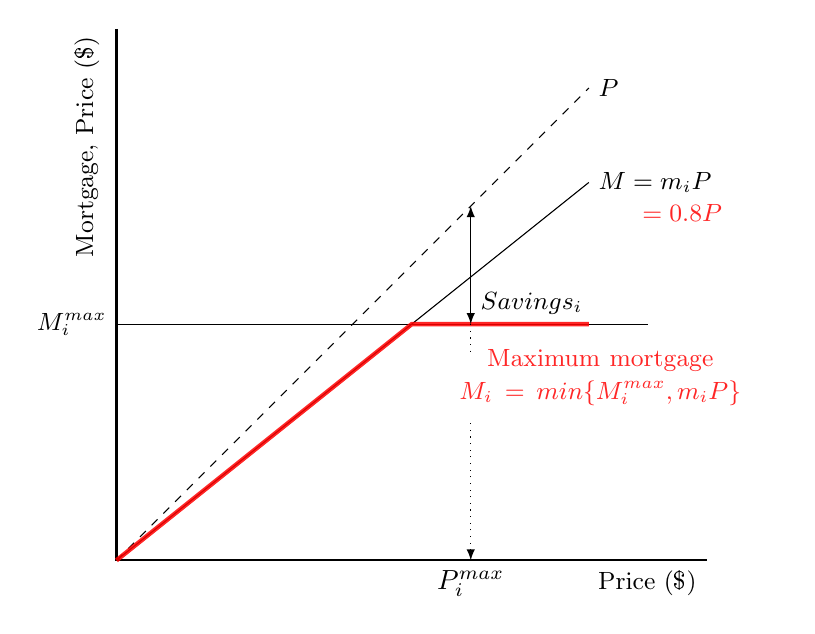
\begin{tikzpicture}	[scale=1.5]
%AXES
\draw[thick] (0,4.5) --(0,0)--(5,0)node[below left]{\small Price (\$)};
\node at (-.25, 3.5)[ rotate=90]{\small Mortgage, Price (\$)};
% M =Mi MAX
\draw[dashed] (0,0)--(4,4)node[right]{\small $P$};
\draw[] (0,2)node[left]{\small $M_i^{max}$}--(4.5,2);%node[right, red]{\small $M = M_i^{max}$};
% M =m_i MAX
%\draw[dotted,red, opacity=.5] (0,0)--(4,3.6)node[right]{\small $M = 0.9P$};
\draw[] (0,0)--(4,3.2)node[right]{\small $M = m_iP$};
\node at(4.37,3.1)[below right, red, opacity=.85 ]{\small $= 0.8P$};
% COMBINED MAX RED
\draw[ultra thick, red, opacity=.85] (0,0)--(2.5,2)node[below right,  text width=4.5cm, align = center]{\small \\ Maximum mortgage \\ $M_i=min\{M_i^{max}, m_iP\}$}--(4.0,2);
% SAVINGS
\draw[latex-latex] (3,2)node[above right] {\small $Savings_i$}--(3,3);
% PMAX
\draw[dotted,latex- ] (3,0)node[below] {$P_i^{max}$}--(3,1.2);
\draw[dotted ] (3,2)--(3,1.72);
\end{tikzpicture}